\section{Auswertung}
Um zu verstehen, welchen Einfluss die Signallaufzeiten in der Schaltung haben,
wurde die Verzögerung dar Signale, die von den beiden zu SC2 gehörenden
Photomultipliern PM2 und PM4 ausgehen, mit einem Oszilloskop gemessen. Dabei
erhielten wir Bilder wie das in \fref{koinzidenz} dargestellte. 

\begin{figure}[htb]
   \centering
   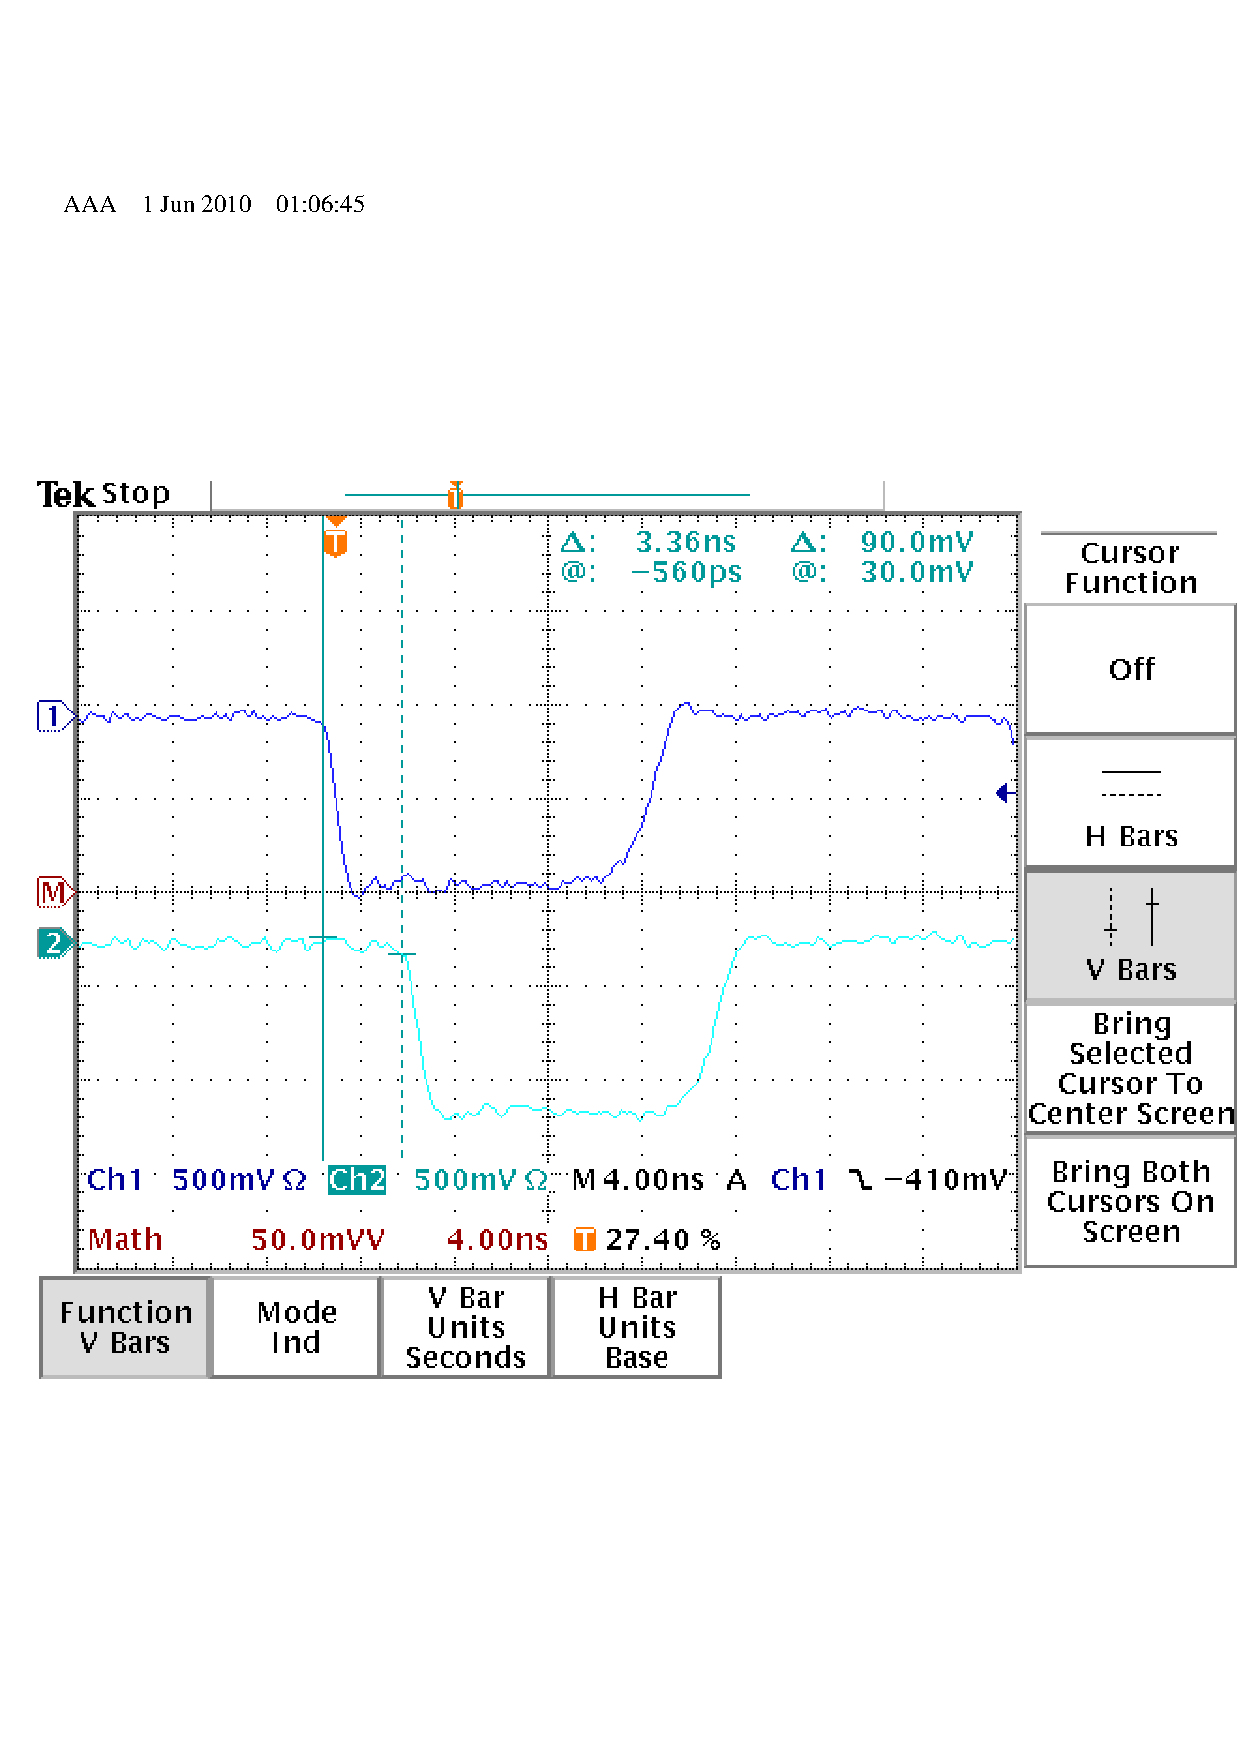
\includegraphics[width=1\columnwidth,keepaspectratio]{../data/TEK00010.pdf}
   \caption{Verzögerung in einer Koinzidenzeinheit}
   \label{fig:koinzidenz}
\end{figure}

Die Verzögerung wurde mit Hilfe der Positionsmarken, die zur Funktionalität des
Oszilloskops gehören, abgelesen, indem diese jeweils an den Beginn des Abfalls
der jeweiligen Kurve gefahren wurden. Die Differenz ist im oberen Bildteil in
der mit $\Delta:$ beginnenden Zeile abzulesen. Wir haben diese Messung sechs
mal durchgeführt. Die Zeitdifferenzen $t_i$ sind in \tref{diff} dargestellt.

\begin{table}[htbp]
\centering
% \setlength{\tabcolsep}{14pt}
\begin{tabular*}{\columnwidth}{%
S[tabformat=1.2]%
S[tabformat=1.2]%
S[tabformat=1.2]%
S[tabformat=1.2]%
S[tabformat=1.2]%
S[tabformat=1.2]%
S[tabformat=2.1]%
}
\toprule
% daten aus ../data/TEK00006.pdf bis 12
{$t_1$} & {$t_2$} & {$t_3$} & {$t_4$} & {$t_5$} & {$t_6$} & {$t_7$}\\
\midrule
3,36 & 4,24 & 0,880 & 8,56 & 0,240 & 0,640 & 24,2\\
\bottomrule
\end{tabular*}
\caption{Messwerte der Verzögerungszeiten (angegeben in ns)}
\label{tab:diff}
\end{table}

Die Unsicherheiten der Zeiten liegen (je nach Messbereich) bei einem oder zwei
LSD (last significant digit). Wie man erkennen kann, schwanken die Zahlen
stark, was daran liegt, dass hier noch gar keine Ereignisselektion
stattgefunden hat und somit alle möglichen Events betrachtet wurden. Man kann
aber auch sehen, dass manche Zeitdifferenzen im Bereich von etwa
\SI{0,2}{\nano\second} liegen, also auf jeden Fall vernachlässigbar gegenüber
den Unsicherheiten der anderen Komponenten sind, zumal man davon ausgehen kann,
dass gerade diese Events diejenigen sind, die in Wirklichkeit gleichzeitig
stattfanden. Die Verzögerung wird also in diesem Bereich liegen.